\documentclass[tikz]{standalone}

\begin{document}
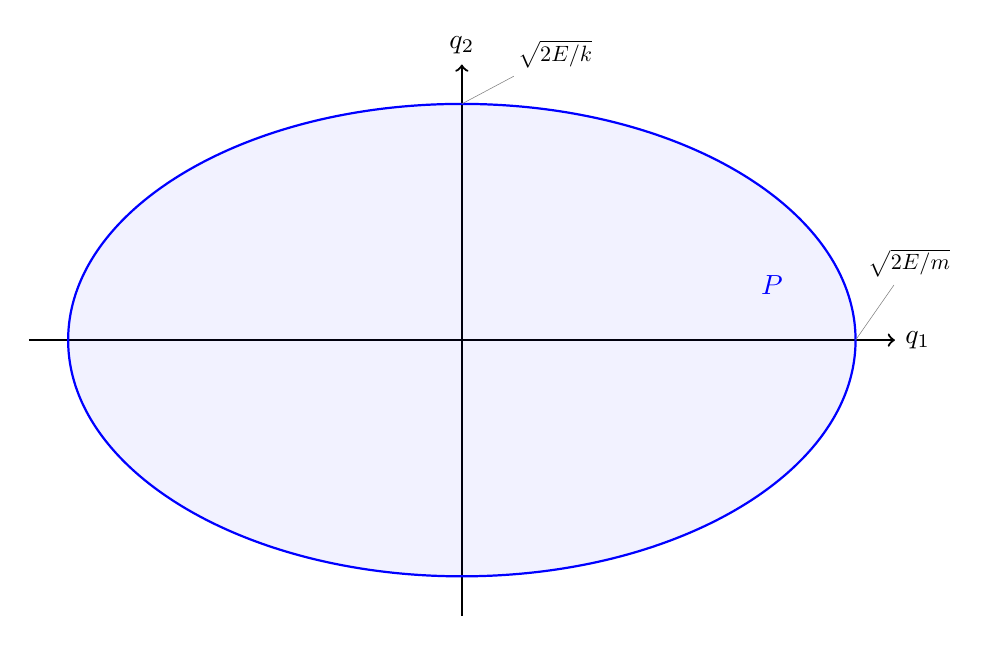
\begin{tikzpicture}[thick]

  % Axes
  \def\x{5}\def\y{3}
  \draw[->] (-\x-0.5,0) -- (\x+0.5,0) node[right] {$q_1$};
  \draw[->] (0,-\y-0.5) -- (0,\y+0.5) node[above] {$q_2$};

  % Ellipse
  \draw[blue,fill=blue,fill opacity=0.05] (0,0) circle [x radius=\x, y radius=\y];
  \coordinate[pin={[pin distance=25,scale=0.8]85:$\sqrt{2E/m}$}] (r1) at (\x,0);
  \coordinate[pin={[pin distance=25,scale=0.8]30:$\sqrt{2E/k}$}] (r2) at (0,\y);
  \node[blue] at (10:\x-1) {$P$};

\end{tikzpicture}
\end{document}